\documentclass[12pt]{article}

\usepackage[pdftex]{graphicx}
\usepackage{times}
\usepackage{xfrac}
\usepackage{longtable}
\usepackage{booktabs}
\usepackage{hyperref}

\topmargin 0.0cm
\oddsidemargin 0.2cm
\textwidth 16cm 
\textheight 21cm
\footskip 1.0cm

\providecommand{\tightlist}{%
  \setlength{\itemsep}{0pt}\setlength{\parskip}{0pt}}

\newlength{\cslhangindent}
\setlength{\cslhangindent}{1.5em}
\newenvironment{cslreferences}%
  {\setlength{\parindent}{0pt}%
  \everypar{\setlength{\hangindent}{\cslhangindent}}\ignorespaces}%
  {\par}

\title{Evaluating the relationships between author reputation and single-blind peer review}

\author{Eitan Frachtenberg, Kelly McConville}



\begin{document}
\maketitle

\begin{abstract}
  \ldots{}
\end{abstract}

\hypertarget{sec:intro}{%
\section{Introduction}\label{sec:intro}}

Numerous studies attempt to answer the question of whether prestige bias exists in the peer review process for a particular discipline of science {[}1{]}--{[}8{]}.
This paper began as one of these studies, focusing on the field of computer systems.
We soon realized that our particular dataset was insufficient to provide conclusive evidence for or against prestige bias.
We also realized that the limitations we encountered may actually be shared by many of these studies and had not been well documented before.
The main focus of our study thus became the exploration of how subtle changes in the data and methods used to detect prestige bias can radically change the resulting outcome.

But first, what is prestige bias, and why should we care about it?
Scientists normally publish their findings in peer-reviewed venues such as journals and conferences.
Their work is judged by a small set of peers from their field, who typically remain anonymous so that their critique can remain free from author influence.
This so-called single-blind (SB) reviewing has been widely accepted as the baseline standard of credibility in the scientific process {[}9{]}.
However, single-blind reviewing still lets reviewers know the identities of the work's authors.
Several researchers have argued that this knowledge can affect the review outcomes in subjective ways.
In particular, when reviewers encounter a famous author or affiliation they may subconsciously experience authority bias, where higher accuracy is attributed to the opinion of authority figures {[}10{]}.
This bias, also known as ``the halo effect'', ``status bias'', or ``prestige bias'', the term we use in this paper.
It has been implicated as an important but unscientific factor in the review process, which in turn can lead to bad science, lower credibility for the scientific process as a whole, and an exacerbation of the underrepresentation of minorities in research {[}8{]}.

A commonly suggested antidote to prestige bias is double-blind (DB) reviewing, where authors' identities and affiliations are hidden from reviewers.
Not all venues employ DB reviewing, both for practical and principled considerations.
However, the coexistence of SB and DB reviewing (sometimes in the same venue) opens the door to comparative studies of the effects of prestige bias.
For example, the association between reviewing policy and various biases has been assessed in fields as disparate as economics {[}blank91:blind{]}, behavioral ecology {[}1{]}, {[}2{]}, ophthalmology {[}4{]}, medicine {[}3{]}, {[}5{]}, psychology {[}6{]}, and computer science {[}7{]}, {[}8{]}.
Some of these studies have found conclusive evidence for bias while others have found no evidence of bias, sometimes in the same field.
Often, these studies were not directly comparable because of various differences in the data, methodologies, or metrics used.
One limitation of these studies is that there are various ways to estimate a person's name recognition, and they all likely yield different results.
Another limitation is that the reviewing policy of a venue is not always independent from other factors, so DB reviewing could be confounded with other factors that affect submission or acceptance decisions.
When we tried to apply similar methodologies to another broad field of research, computer systems, we discovered that the outcome can vary significantly based on the methodology and metrics used.

The main contribution of this paper is therefore an analysis of the sensitivity of the association between reviewing policy and prestige bias.
To emphasize, this study does not attempt to directly address the question of the existence of prestige bias in this field.
Instead, we focus on exposing and analyzing the factors that could change the outcomes of studies that do attempt to address this question.
These factors include questions such as: how to estimate the prestige or reputation of authors? where should data be sourced from, and how should it be cleaned? and how should we correct for confounding variables like conference prestige?
A meaningful analysis of review bias requires a careful consideration of these factors, and a cognizant effort to address the sensitivity of the outcomes to these choices.
Understanding these factors can help accomplish more reliable and stable results in future studies on bias in general, and prestige bias in particular.

The rest of this paper is organized as follows.
We start by describing the extensive dataset we collected on our field of focus in Sec. \ref{sec:data}.
As is often the case with real-world data, it is noisy and contains significant outliers.
We describe the treatment of these outliers and the cleaning of this dataset in general in Sec. \ref{sec:cleaning}.
The next section then describes empirical evidence for and against prestige bias, varying based on the types of metrics and statistical analyses performed.
This section demonstrates how contradictory but statistically significant results can be obtained by different approaches, despite working on the very same dataset.
We elaborate and discuss these findings and practical recommendations in Sec. \ref{sec:discussion}.
Finally, we review related work in Sec. \ref{sec:related} and conclude in Sec. \ref{sec:conclusion}.

\hypertarget{sec:data}{%
\section{Materials and methods}\label{sec:data}}

The primary dataset we analyze comes from a hand-curated collection of 56 peer-reviewed systems conferences from a single publication year (2017).
In CS, and in particular in its more applied fields such as systems, original scientific results are typically first published in peer-reviewed conferences {[}11{]}--{[}14{]}, and then possibly in archival journals, sometimes years later {[}15{]}.
The conferences we selected include some of the most prestigious systems conferences (based on indirect measurements such as Google Scholar's metrics), as well as several smaller or less-competitive conferences for contrast (Table \ref{tab:sys-confs}).
We chose to focus on a large cross-sectional set of conferences from a single publication year (2017), to reduce variations in time.
Our choice of which conferences belong to ``systems'' is necessarily subjective.\footnote{For the purpose of this study, we define systems as the study and engineering of concrete computing systems, which includes research topics such as: operating systems, computer architectures, data storage and management, compilers, parallel and distributed computing, and computer networks.}
Not all systems papers from 2017 are included in our set, and some papers that are in our set may not necessarily be considered part of systems (for example, if they lean more towards algorithms or theory).
However, we believe that our cross-sectional set is both wide enough to represent the field well and focused enough to distinguish it from the rest of CS.
In total, our sample includes 2439 accepted peer-reviewed papers.

\begin{table}

\caption{\label{tab:sys-confs}System conferences, including start date, number of published papers, total number of named authors, acceptance rate, and country code.}
\centering
\fontsize{8}{10}\selectfont
\begin{tabular}[t]{|lcrrr||lcrrr|}
\toprule
Conference & Date & Papers & Authors & Acceptance & Conference & Date & Papers & Authors & Acceptance\\
\midrule
ASPLOS & 2017-04-08 & 56 & 247 & 0.18 & ISC & 2017-06-18 & 22 & 99 & 0.33\\
ATC & 2017-07-12 & 60 & 279 & 0.22 & ISCA & 2017-06-24 & 54 & 295 & 0.17\\
CCGrid & 2017-05-14 & 72 & 296 & 0.25 & ISPASS & 2017-04-24 & 24 & 98 & 0.30\\
CCS & 2017-10-31 & 151 & 589 & 0.18 & KDD & 2017-08-15 & 64 & 237 & 0.09\\
CIDR & 2017-01-08 & 32 & 213 & 0.41 & MASCOTS & 2017-09-20 & 20 & 75 & 0.24\\
CLOUD & 2017-06-25 & 29 & 110 & 0.26 & MICRO & 2017-10-16 & 61 & 306 & 0.19\\
Cluster & 2017-09-05 & 65 & 273 & 0.30 & Middleware & 2017-12-11 & 20 & 91 & 0.26\\
CoNEXT & 2017-12-13 & 32 & 145 & 0.19 & MobiCom & 2017-10-17 & 35 & 164 & 0.19\\
EuroPar & 2017-08-30 & 50 & 179 & 0.28 & NDSS & 2017-02-26 & 68 & 327 & 0.16\\
EuroSys & 2017-04-23 & 41 & 169 & 0.22 & NSDI & 2017-03-27 & 42 & 203 & 0.16\\
FAST & 2017-02-27 & 27 & 119 & 0.23 & OOPSLA & 2017-10-25 & 66 & 232 & 0.30\\
HCW & 2017-05-29 & 7 & 27 & 0.47 & PACT & 2017-09-11 & 25 & 89 & 0.23\\
HiPC & 2017-12-18 & 41 & 168 & 0.22 & PLDI & 2017-06-18 & 47 & 173 & 0.15\\
HotCloud & 2017-07-10 & 19 & 64 & 0.33 & PODC & 2017-07-25 & 38 & 101 & 0.25\\
HotI & 2017-08-28 & 13 & 44 & 0.33 & PODS & 2017-05-14 & 29 & 91 & 0.29\\
HotOS & 2017-05-07 & 29 & 112 & 0.31 & PPoPP & 2017-02-04 & 29 & 122 & 0.22\\
HotStorage & 2017-07-10 & 21 & 94 & 0.36 & SC & 2017-11-13 & 61 & 325 & 0.19\\
HPCA & 2017-02-04 & 50 & 215 & 0.22 & SIGCOMM & 2017-08-21 & 36 & 216 & 0.14\\
HPCC & 2017-12-18 & 77 & 287 & 0.44 & SIGIR & 2017-08-07 & 78 & 264 & 0.22\\
HPDC & 2017-06-28 & 19 & 76 & 0.19 & SIGMETRICS & 2017-06-05 & 27 & 101 & 0.13\\
ICAC & 2017-07-18 & 14 & 46 & 0.19 & SIGMOD & 2017-05-14 & 96 & 335 & 0.20\\
ICDM & 2017-11-19 & 72 & 268 & 0.09 & SLE & 2017-10-23 & 24 & 68 & 0.42\\
ICPE & 2017-04-22 & 29 & 102 & 0.35 & SOCC & 2017-09-25 & 45 & 195 & NA\\
ICPP & 2017-08-14 & 60 & 234 & 0.29 & SOSP & 2017-10-29 & 39 & 217 & 0.17\\
IGSC & 2017-10-23 & 23 & 83 & NA & SP & 2017-05-22 & 60 & 287 & 0.14\\
IISWC & 2017-10-02 & 31 & 121 & 0.37 & SPAA & 2017-07-24 & 31 & 84 & 0.24\\
IMC & 2017-11-01 & 28 & 124 & 0.16 & SYSTOR & 2017-05-22 & 16 & 64 & 0.34\\
IPDPS & 2017-05-29 & 116 & 447 & 0.23 & VEE & 2017-04-09 & 18 & 85 & 0.42\\
\bottomrule
\end{tabular}
\end{table}

To address decisively the question of prestige bias in computer systems, we would need to compare the prestige of accepted authors to that of rejected authors, for which we have no information.
The information we collected measures publication rates for authors, not acceptance rates, so our observations do not lead to conclusive claims on which papers/authors are accepted more.
Higher publication rate of certain authors does not necessarily imply a higher acceptance rate, because, for example, these authors could be submitting more papers to these conferences.
But the two metrics are nevertheless related: all else being equal, a higher acceptance rate will imply a higher publication rate.
So instead, we concentrate not on the existence of prestige bias, but on a related question:
Is there a statistically significant difference in the rates of famous authors published in SB or DB conferences?

To answer this question, we collected extensive information to help us estimate the prestige of authors and conferences.
For each conference, we downloaded all papers and gathered information about all authors, program committee (PC) members, and other roles.
Conferences do not generally offer information on authors' demographics, but we were able to unambiguously link approximately two thirds (65.7\%) of
researchers in our dataset to a Google Scholar (GS) profile.
For each author and PC member, we collected all metrics in their GS profile, such as total previous publications (ca. 2017), h-index, etc.
Note that we found no GS profile for about a third of the researchers
(36.04\%),
and these researchers appear to be less experienced than researchers with a GS profile.
We therefore also another proxy metric for author experience (total number of past publications) from another source, the Semantic Scholar database.

In addition to researcher information, we gathered various statistics on each conference, either from its web page, proceedings, or directly from its chairs.
For each conference, we collected data from the web and from program committee (PC) chairs, including review policies, important dates, the composition of its technical PC, and the number of submitted papers.
We also collected historical metrics from the Institute of Electrical and Electronics Engineers (IEEE), Association for Computing Machinery (ACM), and Google Scholar (GS) websites, including past citations, age, and total publications, and downloaded all 2439 papers.

\hypertarget{statistics}{%
\subsection{Statistics}\label{statistics}}

For statistical testing, group means were compared pairwise using Welch's two-sample t-test; differences between distributions of two categorical variables were tested with \(\chi^{2}\) test; and comparisons between two numeric properties of the same population were evaluated with Pearson's product-moment correlation. All statistical tests are reported with their p-values.

\hypertarget{code-and-data-availability}{%
\subsection{Code and data availability}\label{code-and-data-availability}}

For reproducibility, all of the data and source code files for this paper can be found at \url{https://github.com/eitanf/sysconf/}.

\hypertarget{sec:cleaning}{%
\section{Cleaning the raw data}\label{sec:cleaning}}

\includegraphics{prestige_files/figure-latex/metric-distribs-1.pdf} \includegraphics{prestige_files/figure-latex/metric-distribs-2.pdf}

\begin{figure}
\centering
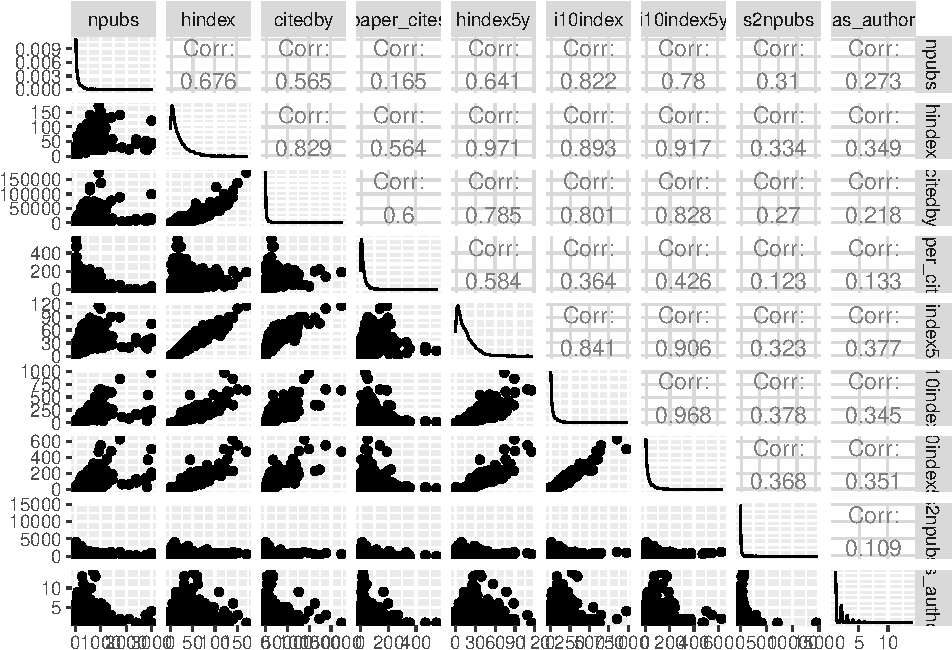
\includegraphics{prestige_files/figure-latex/metric-corrs-1.pdf}
\caption{\label{fig:metric-corrs-1}Correlogram of reputation metrics.}
\end{figure}

\begin{verbatim}
## corrplot 0.87 loaded
\end{verbatim}

\begin{figure}
\centering
\includegraphics{prestige_files/figure-latex/metric-corrs-2.pdf}
\caption{\label{fig:metric-corrs-2}Correlogram of reputation metrics.}
\end{figure}

\begin{itemize}
\tightlist
\item
  All the distributions are right-skewed.
\item
  The two tails have the values we're most worried about: ambiguous names; expansive vs.~minimal inclusion of publications; inexperienced authors with no GS profile.
\item
  Sensitivity analysis
\item
  The correlation between npubs and s2npubs is much higher for ppl.filtered, probably because we removed the points where they disagree by a lot.
\end{itemize}

\hypertarget{sec:results}{%
\section{Empirical results}\label{sec:results}}

In this section we explore the observed relationships between reputation and DB reviewing across three design dimensions, or factors: metrics of reputation, aggregation of prestige across coauthors, and additional conference variables that could affect this relationship. Because of the complexity introduced by multiple independent factors, we start with a commonly set of choices for comparisons and investigate the effect of each factor and level in relation to this baseline. The baseline we chose is to approximate the reputation of a paper's coauthors by the maximum total number of prior publications of any coauthor, and ignoring any confounding variables. This metric has been commonly used in other studies as well {[}3{]}, {[}8{]}, {[}16{]}, {[}17{]}.

\hypertarget{subsec:metrics}{%
\subsection{Reputation metrics}\label{subsec:metrics}}

Author reputation is an intangible, abstract concept. Nevertheless, the quantitative studies that we focus on require a concrete approximation. As a proxy for the intangible reputation, most bibliometric studies employ either metrics based on productivity (publication counts), on impact, (citation metrics), or both {[}18{]}, {[}19{]}. We next describe these metrics and their distributions in our dataset. This list is certainly not exhaustive; the debate on their relative merits and effectiveness is an ongoing research topic, and new and improved metrics are proposed constantly. But this list represents some of the most commonly used metrics, and as our results show, is sufficient to surface problems in the context of reviewing policy.

\hypertarget{publication-counts}{%
\subsubsection{Publication counts}\label{publication-counts}}

Counting the number of past publications is ostensibly the most straightforward way to quantify how well-known an author is. After all, the more papers that carry their name, the more likely it is that their name is recognized by reviewers. But the relationship is hardly linear in practice:

\begin{itemize}
\tightlist
\item
  Not all papers are equally well-known, read, or cited (a problem that the impact-based metrics attempt to address).
\item
  Successful young researchers may be receiving significant name recognition without having yet accumulated a long publication record.
\item
  Deciding what counts as a ``publication'' can be subjective and vary from source to source. For example, do patents count? Arxiv preprints? blog posts?
\item
  Accurate collection of even the raw data is complicated by factors such as author name disambiguation, paper disambiguation, and noisy or crowd-sourced data sources.
\item
  Systems papers in particular vary significantly in numbers of coauthors because some implementations take large team effort. Credit attribution therefore becomes particularly tricky in this field, even with h-index {[}20{]}.
\end{itemize}

We these limitations in mind, we start our analysis by looking at the count of previous publications for each author
For each accepted paper, we looked at the publication count of the most prolific author.
In our dataset, authors in SB conferences average a higher publication count based on GS than in DB conferences
(mean SB: 219.96 DB: 195; \(t=3.06\), \(p=0.00224\)).
This relationship appears to support a hypothesis of prestige bias for these conferences (again, it is insufficient to conclude a causal relationship).
When we compare the publication counts from our other data source, S2, which covers all authors, we find similar evidence, albeit weaker:
(mean SB: 353.05 DB: 312.1; \(t=1.876\), \(p=0.0609\)).

We can also use a third source of paper counts to differentiate between active and mostly inactive researchers, using only up-to-date statistics.
If we look only at the number of papers published in our cross-section of conferences from 2017, we find that SB conference authors actually average significantly fewer publications than those in DB conferences
(mean SB: 2.78 DB: 3.12; \(t=-3.486\), \(p=0.000499\)).
This result could provide evidence against a prestige bias, but it could also point to a completely different hypothesis, such as authors preferring to submit to DB conferences for these specific conferences and point in time.
The evidence based on publication counts alone is inconclusive.

\hypertarget{citation-based-metrics}{%
\subsubsection{Citation-based metrics}\label{citation-based-metrics}}

We next turn our attention to another set of commonly used metrics, those incorporating citations, which is one measure of impact.
Citation-based metrics try to capture the fact that not all publications have the same influence on other researchers, and indirectly, on the author's reputation.
Note that the correlation between total past citations and total past papers is not particularly high, leading potentially to divergent results when evaluating prestige bias
(Pearson correlation of
\(r=0.65\)
when using GS paper counts,
\(r=0.48\)
with S2 data).

From GS, we collected for each author with an identifiable profile they total number of past citations, h-index, i10-index (number of papers with 10 or more citations), the h-index over the past 5 years and the i10-index over the past 5 years.
We omit the last two metrics from our discussion because of their high correlation with h-index and i10-index, respectively (Fig. \ref{fig:metric-corrs}).
We also computed another metric from these statistics, citations per paper, by dividing total citations with total GS publications.

Once more, we look at the most senior coauthor in each paper group, and compare the averages across SB and DB conferences.
Of these, the citations-per-paper metric shows the strongest association with DB reviewing
(mean SB: 33.59 DB: 44.72; \(t=-6.557\), \(p<0.0001\)).
The h-index metric also is strongly indicated with higher values in DB conferences
(mean SB: 31.76 DB: 34.5; \(t=-2.929\), \(p=0.00343\)).

The total citations metric shows a much weaker association in the same direction
(mean SB: 7707.52 DB: 8401.6; \(t=-1.212\), \(p=0.226\)),
while the i10 metric shows a weak association in the opposite direction
(mean SB: 81.12 DB: 78.86; \(t=0.662\), \(p=0.508\)).

\hypertarget{program-committee-metrics}{%
\subsubsection{Program committee metrics}\label{program-committee-metrics}}

Two other reputation metrics that are not regularly reported or measured are participation of the authors in review roles.
Many comparable studies focus on journal authors, where most reviewers remain unidentified, and editorial boards are relatively small.
But in CS, and systems in particular, where the main publication venue is conferences, most of the peer review is carried out by broad, publicized program committees (PCs).

Participation in a PC is related to an author's reputation in two ways.
First, to be invited to serve in a PC, an author needs to typically be regarded as an authority in the field.
We can extend this intuition to reputation metrics, either as a quantitative one---how many PC in our set an author belongs to---or a qualitative one, simply noting whether they participate in any PC at all.
For the former, we observed that the most senior coauthors in each paper group average marginally more PC roles in DB conferences
(mean SB: 1.17 DB: 1.21; \(t=-0.815\), \(p=0.415\)).
For the latter, we observed an opposite indication: the ratio of papers authored by at least one member of a PC in our set is actually lower for DB conferences than for SB
(63.2\%
vs.~59.6\%;
\(\chi{}^2=3.077\), \(p=0.0794\)).

Second, when a person submits a paper to a specific conference wherein they also serve on the PC, they are quite likely recognized by reviewers, who also compose the PC.
We can compute the percentage of papers in each conference where at least one of the authors participates in the PC for that same conference.
Comparing across review polices, we find no significant difference in the mean percentage for DB and SB conferences
(25\%
vs.~27\%;
\(t=-0.38\), \(p=0.705\)).

In summary, neither of the PC metrics for reputation shows a strong association with the review policy of the conference.

\hypertarget{subsec:aggregation}{%
\subsection{Paper summaries}\label{subsec:aggregation}}

The analysis so far made two implicit assumptions on the likelihood that a paper would be recognized as ``reputable'': that the author with the highest reputation metic determines the reputation of the paper, and that the likelihood increases linearly with the value of the reputation metric.
In this section, we expand our analysis beyond these assumptions.
We first look at the effect of summarizing a paper's author reputation based on other coauthors or author groups.
Then, we look at qualitative (noncontinuous) classifications of a paper's potential for recognition.

\hypertarget{aggregations-by-paper}{%
\subsubsection{Aggregations by paper}\label{aggregations-by-paper}}

The typical systems paper has a large number of coauthors compared to other disciplines, perhaps because of its emphasis on concrete systems that can require significant team effort to implement.
In our dataset, papers average
4.42 authors per paper
(SD: 2.63).
We have assumed so far that a paper is most likely to be recognized based solely on the author with the highest reputation metric.
But other authors may play an important role in name recognition, as well as the whole group.

For example, the total or average reputation of the coauthor group could also play a potential role in the reviewer's bias.
As another example, the typical systems paper lists the primary contributor in the first author position, while the head of the lab is often listed last.
In our dataset, only
12.02\%
of papers with 3 or more coauthors ordered the author list alphabetically.

\begin{figure}
\centering
\includegraphics{prestige_files/figure-latex/mean-diffs-1.pdf}
\caption{\label{fig:mean-diffs}Difference in means for various reputation metrics and aggregations across papers using two-sided Student's t-test. Positive t-statistic values (purple) indicate higher reputation in SB conferences. Negative values (orange) indicate higher reputation in DB conferences. Stars indicate p values below 0.05, 0.01, and 0.001, respectively.}
\end{figure}

Looking at all six aggregation methods across seven reputation metrics reveals a mixed picture (Fig. \ref{fig:mean-diffs}).
The first row (using maximum reputation per paper aggregation) repeats the results we discussed in Sec. \ref{subsec:metrics}.
All other rows represent new aggregations.
Depending on one's choice of metrics and aggregations, one can measure statistically significant reputation bias, anti-bias, or nonsignificant bias.
Any stastically sound evidence to suggest bias can find a counter-argument just as sound in this dataset.

Nevertheless, we can discern a few consistent properties from these comparisons:

\begin{itemize}
\item
  The citations-per-paper and papers-in-set metrics indicate lower mean reputation in SB conferences across all paper aggregations. It is noteworthy because these two metrics are completely unrelated in time: one looks at the past, and one at the present.
\item
  Conversely, measuring reputation by number of publications results in higher mean reputation for SB conferences, regardless of aggregation or database used.
\item
  However, using the more complete S2 database, which includes many more authors of low experience and reputation, lowers the t-statistic values and significance. This result may not be surprising, at it incorporates more data, particularly on the lower side of the reputation distribution; but it serves as a cautionary tale for ascribing statistical significance from partial data.
\item
  Similarly, aggregating papers by the reputation of the lead author results in the least conclusive findings. We believe that many lead authors are relatively inexperienced graduate students.
\item
  Looking at each paper's median reputation metric instead of mean leads to higher t-statistic values, i.e., higher indicated reputation in SB conferences and higer likelihood of prestige bias. (((Why?)))
\end{itemize}

Related to the last point, we can look not only at median aggregation per paper, but also across papers.
That is, we can compare how the median reputation per paper (however it is aggregated) differs between SB and DB conferences, again with the purpose of attenuating the effect of large right-skewed outliers.

\begin{figure}
\centering
\includegraphics{prestige_files/figure-latex/median-diffs-1.pdf}
\caption{\label{fig:median-diffs}Difference in medians for various reputation metrics and aggregations across papers using two-sided Wilcoxon test. Positive values (purple) indicate higher reputation in SB conferences. Negative values (orange) indicate higher reputation in DB conferences. Stars indicate p values (from a Wilcoxon two-sided unpaired test) below 0.05, 0.01, and 0.001, respectively.}
\end{figure}

As Fig. \ref{fig:median-diffs} shows, many of the metrics and paper aggregations agree in direction (sign) whether looking at the mean values across SB/DB or medians, although confidence levels vary significantly between the two.
Observe for example how the total citation metric went from nonsignificant means to highly significant medians, perhaps because this metric's values are the most widely distributed and right-skewed, therefore creating large differences between means and medians.

The implication from this comparison is, again, that there exist combinations of metrics and aggregations, all presumably reasonable choices to make, that can change from statistical significance to nonsignificance.
For example, a 2006 study found no significant difference in the mean publications of authors in two conferences {[}16{]}, but a followup study on the same dataset found evidence for prestige bias when comparing across medians {[}17{]}.
The choices for metrics and aggregations must therefore be carefully justified, compared, and balanced to increase the credibility of such analyses.

\hypertarget{binary-classifications-of-fame}{%
\subsubsection{Binary classifications of fame}\label{binary-classifications-of-fame}}

So far, we have treated the reputation or fame of researchers as a continuous variable.
This treatment allowed us to answer the question of whether the likelihood of an author to publish in SB proceedings increases commensurate with their reputation metrics.
But the question of reputation bias may instead be more binary, based on the accept/reject outcome of a paper: either a paper is accepted based on an author's reputation being recognized or it is not.
This qualitative classification bypasses the problem of the long tails of the reputation metrics that could skew the mean reputation of a sample.

The quantitative question then becomes, what is the proportion of accepted papers in SB and DB conferences for which at least one of the authors carries enough reputation to be recognized?
Since we do not know a-priori what ``enough reputation'' means, we can observe how these proportions change based on different reputation metrics and thresholds.

\begin{figure}
\centering
\includegraphics{prestige_files/figure-latex/rep-threshold-npubs-1.pdf}
\caption{\label{fig:rep-threshold-npubs}Proportion of papers that have at least one author with at least as many publications as the threshold (Google Scholar data).}
\end{figure}

For example, Fig. \ref{fig:rep-threshold-npubs} shows the difference in proportions of papers written by famous authors in SB or DB conferences, based on number of publications.
It shows that beyond a certain level of reputation (around 100 papers), famous authors are always overrepresented in SB conferences, consistent with a possible prestige bias.
Comparing these proportions across SB and DB conferences, with \(\chi{}^2\)-test-derived p-values below 0.05 in 67.8\% of the threshold values.

\begin{figure}
\centering
\includegraphics{prestige_files/figure-latex/rep-threshold-h-1.pdf}
\caption{\label{fig:rep-threshold-h}Proportion of papers that have at least one author with an h-index value above the threshold.}
\end{figure}

The evidence is even stronger when using h-index for reputation, but in reverse.
Fig. \ref{fig:rep-threshold-h} shows that papers by ``famous'' authors in DB conferences consistently outnumber those in SB conferences by an almost-fixed amount of some 5\%--10\%.
This time, p-values below 0.05 show up for 82\% of the threshold values.

These two examples show strong statistical evidence with remarkable insensitivity to the threshold chosen, but in opposite directions.
They demonstrate how critically the conclusion for or against prestige bias can depend on the chosen reputation metric.

\hypertarget{banded-classification-of-seniority}{%
\subsubsection{Banded classification of seniority}\label{banded-classification-of-seniority}}

Another related qualitative approach to look at seniority and experience was described in the original h-index study {[}21{]}. It proposed that researchers may fall into experience bands, roughly corresponding to novice/assistant professor, mid-career/associate professor, and experienced/full professor. Based on his observations of the field of physics, Hirsch suggested h-index limits of up to 11, between 12 and 17, and 18 and over to distinguish among these bands.

\begin{figure}
\includegraphics[width=0.75\textwidth]{prestige_files/figure-latex/seniority-1} \caption{Experience bands of papers' authors by review policy. Each paper is counted exactly once, based on the highest h-index among its coauthors.}\label{fig:seniority}
\end{figure}

When we apply these (admittedly arbitrary) limits to our dataset (Fig. \ref{fig:seniority}), we find a slight advantage to senior researchers in DB reviewed papers
(\(\chi{}^2=6.616\), \(p=0.0366\)).
This anti-prestige bias is consistent with the evidence we uncovered in previous sections using maximum h-index, both for quantitative and qualitative aggregations.

\hypertarget{prestige-by-affiliation}{%
\subsubsection{Prestige by affiliation}\label{prestige-by-affiliation}}

To complete our exploration of paper summaries, we look at one more useful aggregation method to approximate name recognition of authors, based on their affiliation.
For this analysis, we follow the methodology of Tomkins, Zhang, and Heavlin who examined prestige bias in the 2017 Web Search and Data Mining (WSDM) conference {[}8{]}.
Their study tagged a paper as coming from a ``top university'' if any of its coauthors is affiliated with one of the top 50 univsersities per \url{www.topuniversities.com} (27\% of papers).
The similarly tagged a paper as coming from a top company if any author was affiliated with either Google, Microsoft, Yahoo!, or Facebook (18\% of papers).
(It is reasonable to include more companies in the definition of ``top company'' for systems conferences, such as Amazon, Oracle, and Apple, but we kept the same definition for direct comparisons.)

Since our data comes from the same publication year as theirs, it makes sense that we use exactly the same criteria for tagging for an apples-to-apples comparison.
Unfortunately, the original study and supporting information does not contain the list of univiersities or how it was obtained.
We therefore downloaded the list of the top 50 ``Engineering and Technology'' universities and saved it as a list of internet domain names (see supplementary materials, under \texttt{data/top50uni.csv}).

In our dataset,
31.9\%
of papers had at least one coauthor from a top university, and
7.1\%
of papers had at least one coauthor from a top company.
The percentage of papers for authors from a top university in DB conferences is significantly higher than in SB conferences
(33.1\%
vs.~27.5\%,
\(\chi{}^2=8.332\), \(p=0.0039\))
The same can be said for top-company affiliation
(8\%
vs.~4.8\%,
\(\chi{}^2=9.121\), \(p=0.00253\)).

It appears that this aggregation, like total citations or maximum h-index but contrary to Tomkins' results, is consistent with anti-prestige bias (higher prestige in SB conferences).
Unlike Tomkins' results, however, our data does not come from a controlled experiment on a single conference, so cannot provide counterfactual evidence.

\hypertarget{subsec:confounding}{%
\subsection{Confounding variables}\label{subsec:confounding}}

A conference chair's choice to employ DB reviewing is often connected to other conference factors that may also be connected to the experience of researchers submitting to it.
DB conferences tend to have a longer history
(\(t=2.48\), \(p=0.0167\)),
a lower acceptance rate
(\(t=-2.904\), \(p=0.0054\)),
higher H5-index in GS
(\(t=2.786\), \(p=0.00763\)),
longer papers
(\(t=5.01\), \(p<0.0001\)),
more paper submissions
(\(t=2.02\), \(p=0.0495\)),
with more coauthors per paper
(\(t=2.02\), \(p=0.0495\)),
lower ratio of authors coming from the PC itself
(\(t=-2.792\), \(p=0.0076\)),
and more citations to past papers
(\(t=1.489\), \(p=0.145\)),
especially when normalized to citations per paper
(\(t=2.671\), \(p=0.011\)).

In other words, DB conferences themselves show several other distinct characteristics, many of which associated with better reputation. The higher implied prestige of the conference could be associated with the prestige of authors as well, confounding the relationship.
Although we do not have experimental data to infer a causal relationship between the two, the inclusion alone of confounding variables could weaken the observed association between DB conferences and author prestige.
Every one of these variables could potentially serve as a better predictor of author reputation than DB reviewing, which could complicate drawing conclusions on review bias from other observational studies as well.

To evaluate the effect of these confounding variables, we picked the author reputation metric with the strongest relationship to DB reviewing, --- , and recalculated the relationship while correcting for each variable.

Check with logistic regression (glm with method=binomial), contrast with linear model

\hypertarget{sec:discussion}{%
\section{Discussion}\label{sec:discussion}}

-- There are two ``types'' of senior researchers. Type A publish fewer but more cited papers, and type B just publishes a lot of papers, but have lower h-index than type A relative to npubs. The DB conferences show more type-A people, and the SB more type B. The DB conferences also average higher on various prestige metrics and are more competitive. This would be consistent with fewer, more cited papers. But it means you have to correct for conference prestige.

\begin{itemize}
\tightlist
\item
  To demonstrate this, compute for each paper mean citations/paper (for either max\_h person or max\_npubs) and correlate with acceptance rate of conference.
\end{itemize}

-- Effects of other ways of cleaning the data, outliers.

-- Even the same metric, npubs, from different data sources (GS/S2) can yield very different distributions, because each database comes up with its own choices to inherently hard questions like ``what constitutes a publication'' and ``how to disambiguate names''.

-- Recommendations? perhaps any-famous using npubs from a reliable/complete source? Correct for conference prestige by acceptance rate (or whatever the strongest correlate to DB was).

DB reviewing is also associated with fewer authors that are PC members
(\(t=-2.792\), \(p=0.0076\)),
although it has no effect on the number of papers with at least one PC author
(\(t=-0.38\), \(p=0.705\)),
--Could be less PC name recognition on review, but some conferences limit how many papers a PC may submit???

\begin{itemize}
\tightlist
\item
  {[}nicholas17:early{]} Early career researchers appear to have a positive experience overall with peer review. They actually aim for high-impact journals and are influential in choosing where to publish.
\end{itemize}

Figure: scatter plot citations vs.~npubs, color by DB or acceptance rate (or + size) of last authors or all authors. Circle the two groups of ``quality'' and ``quantity''.
It is not surprising that researchers who exhibit few, highly cited papers publish in competitive conferences. It is almost tautological that authors of highly-cited papers publish in highly-cited conferences.
Similarly, it is not surprising that authors with many publications publish in conferences with a lower acceptance rate, regardless of causality.
Therefore, the prevalence of ``famous authors'' in a conference may have more to do with the characteristics of the researcher and conference than with prestige bias, and at any rate is very hard to tease out in an observational study.

\hypertarget{sec:related}{%
\section{Related work}\label{sec:related}}

\hypertarget{prestige-bias-in-peer-review}{%
\subsection{Prestige bias in peer review}\label{prestige-bias-in-peer-review}}

The integrity of the peer-review process is of utmost importance to science and scientists, and is thus an active research area all of its own.
As an inherently human process, influenced by the opinions, perspective, and understanding of human reviewers, peer review is potentially subject to various cognitive biases.
Numerous studies attempt to identify, measure, and offer interventions for such biases.
However, the gold standard for such experiments, randomized controlled trials, is exceedingly difficult to carry out and generalize {[}22{]}--{[}25{]}.
Aside from the usual ethical challenges of experimenting on humans, the properties of the scientific publication make repeatable and controllable experiments particularly difficult.
Papers are typically disallowed from concurrent submission, so A/B experimentation with the same papers is both complex and only partially controlled.
Moreover, actual scientific publications have potentially enormous impact on everyone involved, so the review process cannot be arbitrarily tweaked for the purposes of experimentation.

The upshot of such constraints is that there are relatively few studies on peer-review bias using representative controlled experiments, they are often limited in scope to one journal or conference, and depending on their data and methods, can reach incompatible conclusions {[}8{]}, {[}26{]}, {[}27{]}.
A literature survey from 15 years ago on the question of prestige bias found mixed results {[}28{]}, as have we in the literature since then.

In one famous study, for example, Fisher et al performed a randomized trial on 57 consecutive submissions to the Journal of Development and Behavioral Pediatrics.
Each paper received 2 SB and 2 DB reviews, and acceptance decisions were compared to the number of publications of each paper's lead author and most-senior author.
The paper concludes that SB reviewing favors authors with higher publication counts.

A similar but more recent example experimented on the submissions to the WSDM'17 conference on data mining {[}8{]}.
The experiment split the PC into two halves, one using SB reviewing and the other DB, with two papers from each PC reviewing each paper.
The study looked at the following covariates: author gender; sector of majority coauthors per paper; most common country of majority coauthors; country homophily with reviewers (we don't have that info); famous author (based on a criterion of at least 100 past publications, 3 of which in WSDM); and affiliation prestige (based on top-50 university list or top-4 company list).
Their findings suggest a strong bias in favor of authors with individual or affiliation prestige in SB reviews.
The paper also acknowledges the difficulty and rarity of such controlled experiments and points out to a single other study {[}29{]}.
As Tomkins et al summarize:

\begin{quote}
Perhaps the best-known experimental study of SB vs.~DB reviewing behavior, and to our knowledge the only controlled experiment in this area other than our own, is the study by Rebecca Blank (15). Over several years, 1,498 papers were randomly assigned to SB vs.~DB reviewing condition. While Blank performs detailed analyses of many facets of the data, we may summarize part of the high-level findings as follows. First, authors at top or bottom institutions do not see significant differences in acceptance decisions based on reviewing model, but authors at midtier institutions perform better in a SB setting, as do foreign authors and those out-side academia. Second, there is a mild indication, not statistically significant, that women do slightly better in DB review. {[}8{]}
\end{quote}

A different experimental approach, using a fabricated article listing two famous researchers as authors, found that ``Reviewers were more likely to recommend acceptance when the prestigious authors' names and institutions were visible\ldots{} than when they were redacted\ldots{} and also gave higher ratings for the methods and other categories'' {[}5{]}.

Yet another approach, with controversial ethical considerations, was reported in an study that retitled and resubmitted 12 famous papers in psychology with fictitious authors and institutes {[}6{]}.
Three of those were detected as resubmissions, and eight of the remaining nine were rejected in SB peer review.

Closer to our field of study, Madden and DeWitt {[}16{]} looked retrospectively at VLDB and SIGMOD conference papers (SIGMOD is also in our dataset).
Similar to our approach, this observational study did not look at rejected papers or experiment with the review process itself.
While our study compares the publication ratios of famous authors across SB/DB conferences in the same field and point in time, this study compares them across time for the same two conferences, before and after they switched from SB to DB reviewing.
For the purpose of their study, ``famous authors'' were defined as those 25 ``prolific'' individuals with at least 20 past publications in these two conferences, including recent publications.
The comparison found that the mean publication rate of famous authors was substantially the same for SB years and DB years.

Interestingly, a followup analysis on the same dataset came to a contrary conclusion by simply comparing median publication rates instead of means {[}17{]}.
The justification for using medians was that it is more robust to outliers, which for this dataset was particularly relevant because only one of the measured values fell above the mean.
This study not only demonstrates the sensitivity of similar conclusions to the metrics used, as we show as well, but also cautions that ``here are probably a lot of other factors that must be taken into consideration before the database community makes a final choice on whether to continue with double blind review.''

\hypertarget{prestige-metrics}{%
\subsection{Prestige metrics}\label{prestige-metrics}}

Since we found no consensus in the literature on the existence of prestige bias in SB reviewing, or even on the methods to measure it, could we at least found a common answer to the smaller question, ``how should we quantify research prestige?''

Unfortunately, we found no such answer either.
The field of bibliometrics is rich with studies comparing different and contradictory metrics to evaluate the productivity, prestige, and impact of scientific work and researchers, and we can only review a fraction of this discussion in the scope of this paper.

The highly influential h-index, for example, was proposed to combine productivity with echo, and to address specific shortcomings of the publications and citations count metrics, such as sensitivity to a single highly-cited paper (``one-hit wonders'') and prolific authors in low-quality venues {[}21{]}, {[}30{]}, {[}31{]}.

But some researchers argue that a few influential papers should count more than a bevy of poorly cited papers {[}31{]}, {[}32{]} and that h-index is overly sensitive to the length of a researcher's career {[}33{]}.

Furthermore, the h-index has additional shortcomings of its own.
It can be inconsistent {[}34{]}, or be manipulated with self-citations {[}35{]}.
It also does not account properly for the magnitude of individual contributions in team papers {[}20{]}, {[}31{]}.
This criticism applies to the total publications metric as well, and most other widely used reputation metrics.
Finally, even when deciding to use h-index, several studies found different counts in different databases (as have we).
They caution that more than one source should be used to compute h-index accurately, and that comparisons between researchers should be limited to the same data source {[}36{]}, {[}37{]}.

Other citation-based reputation metrics have been proposed to overcome some of these limitations, such as g-index {[}32{]}, p-index {[}38{]}, I3 {[}39{]}, AR-index {[}40{]}, and even simply total citations.
All of these metrics have been found to correlate with each other (as we have also observed) and are generally sensitive to changes in number of publications as well {[}41{]}, {[}42{]}.
In fact, Bertoli-Barsotti and Lando built a model to predict one reputation metric based on the others, which shows that the relationships between metrics can be complex and nonlinear {[}43{]}.
These relationships and model mean that most metrics are codependent, so adding reputation metrics to evaluate bias may not add as much signal as desired.

Nevertheless, we believe that it would be wrong to focus on a single metric without performing a sensitivity analysis with additional metrics that may provide counterevidence.
Carpenter et al also concluded, based on a comparison of traditional and emerging publication metrics, that no single metric is descriptive enough {[}18{]}.
Instead, they suggest that a complete picture of author reputation includes multiple metrics, including traditional productivity- and impact-level metrics, as well as document-level metrics such as views, downloads, tweets, and translations.
Standardizing and incorporating such \emph{altmetrics} as part of an author's reputation or name recognition could potentially improve the analyses of prestige bias in peer review.

\hypertarget{sec:conclusion}{%
\section{Conclusion}\label{sec:conclusion}}

Randomized controlled trials are the gold standard for social experiments, such as those trying to evaluate the peer review system.
These trials clearly require cognizant choices of control covariates and metrics.
In practice, various practical and ethical challenges mean that such trials are often infeasible for evaluating bias, necessitating obervational studies.
These studies also require the same careful consideration for metrics and control variables.
Our analysis showed that \ldots{}

\begin{itemize}
\tightlist
\item
  Add recommendations? perhaps to discussion?
\item
  Nearly all the metrics tested show higher prestige in single-blind, suggesting prestige bias.
\item
  The only exception is the metric max h-index (h-index of most senior author per paper), which is lower in single-blind (p=0.0055).
\item
  This reversal isn't changed whether we drop the NA h-index, flatten them, or linearly impute them from \# papers or S2npubs (at least for median; also for mean when eliminating extremely high imputed values).
\item
  The higher prestige bias survives when controlling for conference prestige (either with h5\_hindex or with I(mean\_historical\_citations/age)). But not when controlling for pc\_author\_ratio and pc\_paper\_ratio.
\end{itemize}

We hope that this paper provides a guideline and a roadmap to studies on bias on how to carefully address methodological issues that could limit the generalization or credibility of their results.

\hypertarget{acknowledgements}{%
\subsubsection*{Acknowledgements}\label{acknowledgements}}
\addcontentsline{toc}{subsubsection}{Acknowledgements}

\hypertarget{references}{%
\section*{References}\label{references}}
\addcontentsline{toc}{section}{References}

\hypertarget{refs}{}
\leavevmode\hypertarget{ref-budden08:double}{}%
{[}1{]} A. E. Budden, T. Tregenza, L. W. Aarssen, J. Koricheva, R. Leimu, and C. J. Lortie, ``Double-blind review favours increased representation of female authors,'' \emph{Trends in ecology \& evolution}, vol. 23, no. 1, pp. 4--6, 2008.

\leavevmode\hypertarget{ref-cox19:cases}{}%
{[}2{]} A. R. Cox and R. Montgomerie, ``The cases for and against double-blind reviews,'' \emph{PeerJ}, vol. 7, p. e6702, 2019.

\leavevmode\hypertarget{ref-fisher94:effects}{}%
{[}3{]} M. Fisher, S. B. Friedman, and B. Strauss, ``The effects of blinding on acceptance of research papers by peer review,'' \emph{JAMA}, vol. 272, no. 2, pp. 143--146, 1994.

\leavevmode\hypertarget{ref-kalavar21:single}{}%
{[}4{]} M. Kalavar, A. Watane, D. Wu, J. Sridhar, P. Mruthyunjaya, and R. Parikh, ``Single-blind and double-blind peer review: Effects on national representation,'' in \emph{Seminars in ophthalmology}, 2021, pp. 1--6.

\leavevmode\hypertarget{ref-okike16:single}{}%
{[}5{]} K. Okike, K. T. Hug, M. S. Kocher, and S. S. Leopold, ``Single-blind vs double-blind peer review in the setting of author prestige,'' \emph{JAMA}, vol. 316, no. 12, pp. 1315--1316, 2016.

\leavevmode\hypertarget{ref-peters82:peer}{}%
{[}6{]} D. P. Peters and S. J. Ceci, ``Peer-review practices of psychological journals: The fate of published articles, submitted again,'' \emph{Behavioral and Brain Sciences}, vol. 5, no. 2, pp. 187--195, 1982.

\leavevmode\hypertarget{ref-seeber17:newcomers}{}%
{[}7{]} M. Seeber and A. Bacchelli, ``Does single blind peer review hinder newcomers?'' \emph{Scientometrics}, vol. 113, no. 1, pp. 567--585, 2017.

\leavevmode\hypertarget{ref-tomkins17:reviewer}{}%
{[}8{]} A. Tomkins, M. Zhang, and W. D. Heavlin, ``Reviewer bias in single-versus double-blind peer review,'' \emph{Proceedings of the National Academy of Sciences}, vol. 114, no. 48, pp. 12708--12713, 2017.

\leavevmode\hypertarget{ref-hames08:peer}{}%
{[}9{]} I. Hames, \emph{Peer review and manuscript management in scientific journals: Guidelines for good practice}. Malden, MA: Blackwell Publishing, 2008.

\leavevmode\hypertarget{ref-ramos17:biases}{}%
{[}10{]} V. J. Ramos, \emph{Analyzing the role of cognitive biases in the decision making process}. Information Science Reference, 2017.

\leavevmode\hypertarget{ref-franceschet10:role}{}%
{[}11{]} M. Franceschet, ``The role of conference publications in CS,'' \emph{Communications of the ACM}, vol. 53, no. 12, pp. 129--132, Dec. 2010.

\leavevmode\hypertarget{ref-freyne10:relative}{}%
{[}12{]} J. Freyne, L. Coyle, B. Smyth, and P. Cunningham, ``Relative status of journal and conference publications in computer science,'' \emph{Communications of the ACM}, vol. 53, no. 11, pp. 124--132, 2010.

\leavevmode\hypertarget{ref-patterson99:evaluating}{}%
{[}13{]} D. Patterson, L. Snyder, and J. Ullman, ``Evaluating computer scientists and engineers for promotion and tenure,'' \emph{Computing Research News}, 1999.

\leavevmode\hypertarget{ref-vardi09:conferences}{}%
{[}14{]} M. Y. Vardi, ``Conferences vs. Journals in computing research,'' \emph{Communications of the ACM}, vol. 52, no. 5, pp. 5--5, 2009.

\leavevmode\hypertarget{ref-vrettas15:conferences}{}%
{[}15{]} G. Vrettas and M. Sanderson, ``Conferences versus journals in computer science,'' \emph{Journal of the Association for Information Science and Technology}, vol. 66, no. 12, pp. 2674--2684, 2015.

\leavevmode\hypertarget{ref-madden06:impact}{}%
{[}16{]} S. Madden and D. DeWitt, ``Impact of double-blind reviewing on sigmod publication rates,'' \emph{ACM SIGMOD Record}, vol. 35, no. 2, pp. 29--32, 2006.

\leavevmode\hypertarget{ref-tung06:impact}{}%
{[}17{]} A. K. Tung, ``Impact of double blind reviewing on sigmod publication: A more detail analysis,'' \emph{ACM SIGMOD Record}, vol. 35, no. 3, pp. 6--7, 2006.

\leavevmode\hypertarget{ref-carpenter14:metrics}{}%
{[}18{]} C. R. Carpenter, D. C. Cone, and C. C. Sarli, ``Using publication metrics to highlight academic productivity and research impact,'' \emph{Academic emergency medicine}, vol. 21, no. 10, pp. 1160--1172, 2014.

\leavevmode\hypertarget{ref-dettori19:measuring}{}%
{[}19{]} J. R. Dettori, D. C. Norvell, and J. R. Chapman, ``Measuring academic success: The art and science of publication metrics,'' \emph{Global spine journal}, vol. 9, no. 2, pp. 243--246, 2019.

\leavevmode\hypertarget{ref-koltun21:hindex}{}%
{[}20{]} V. Koltun and D. Hafner, ``The h-index is no longer an effective correlate of scientific reputation,'' \emph{arXiv preprint arXiv:2102.03234}, 2021.

\leavevmode\hypertarget{ref-hirsch05:index}{}%
{[}21{]} J. E. Hirsch, ``An index to quantify an individual's scientific research output,'' \emph{Proceedings of the National academy of Sciences}, vol. 102, no. 46, pp. 16569--16572, 2005.

\leavevmode\hypertarget{ref-beverly13:findings}{}%
{[}22{]} R. Beverly and M. Allman, ``Findings and implications from data mining the IMC review process,'' \emph{ACM SIGCOMM Computer Communication Review}, vol. 43, no. 1, pp. 22--29, 2013.

\leavevmode\hypertarget{ref-ernst94:reviewer}{}%
{[}23{]} E. Ernst and K.-L. Resch, ``Reviewer bias: A blinded experimental study,'' \emph{The Journal of laboratory and clinical medicine}, vol. 124, no. 2, pp. 178--182, 1994.

\leavevmode\hypertarget{ref-mahoney77:publication}{}%
{[}24{]} M. J. Mahoney, ``Publication prejudices: An experimental study of confirmatory bias in the peer review system,'' \emph{Cognitive therapy and research}, vol. 1, no. 2, pp. 161--175, 1977.

\leavevmode\hypertarget{ref-mcnutt90:blinding}{}%
{[}25{]} R. A. McNutt, A. T. Evans, R. H. Fletcher, and S. W. Fletcher, ``The effects of blinding on the quality of peer review: A randomized trial,'' \emph{JAMA}, vol. 263, no. 10, pp. 1371--1376, 1990.

\leavevmode\hypertarget{ref-parno17:SPsurvey}{}%
{[}26{]} B. Parno, U. Erlingsson, and W. Enck, ``Report on the IEEE S\&P 2017 submission and review process and its experiments.'' 2017.

\leavevmode\hypertarget{ref-shah18:design}{}%
{[}27{]} N. B. Shah, B. Tabibian, K. Muandet, I. Guyon, and U. Von Luxburg, ``Design and analysis of the NIPS 2016 review process,'' \emph{The Journal of Machine Learning Research}, vol. 19, no. 1, pp. 1913--1946, 2018.

\leavevmode\hypertarget{ref-snodgrass06:single}{}%
{[}28{]} R. Snodgrass, ``Single-versus double-blind reviewing: An analysis of the literature,'' \emph{ACM SIGMOD Record}, vol. 35, no. 3, pp. 8--21, 2006.

\leavevmode\hypertarget{ref-blank91:effects}{}%
{[}29{]} R. M. Blank, ``The effects of double-blind versus single-blind reviewing: Experimental evidence from the american economic review,'' \emph{The American Economic Review}, pp. 1041--1067, 1991.

\leavevmode\hypertarget{ref-bornmann07:hindex}{}%
{[}30{]} L. Bornmann and H.-D. Daniel, ``What do we know about the h index?'' \emph{Journal of the American Society for Information Science and technology}, vol. 58, no. 9, pp. 1381--1385, 2007.

\leavevmode\hypertarget{ref-masic16:scientometric}{}%
{[}31{]} I. Masic and E. Begic, ``Scientometric dilemma: Is h-index adequate for scientific validity of academic's work?'' \emph{Acta Informatica Medica}, vol. 24, no. 4, p. 228, 2016.

\leavevmode\hypertarget{ref-egghe06:theory}{}%
{[}32{]} L. Egghe, ``Theory and practise of the g-index,'' \emph{Scientometrics}, vol. 69, no. 1, pp. 131--152, 2006.

\leavevmode\hypertarget{ref-vinkler07:eminence}{}%
{[}33{]} P. Vinkler, ``Eminence of scientists in the light of the h-index and other scientometric indicators,'' \emph{Journal of information science}, vol. 33, no. 4, pp. 481--491, 2007.

\leavevmode\hypertarget{ref-waltman12:inconsistency}{}%
{[}34{]} L. Waltman and N. J. Van Eck, ``The inconsistency of the h-index,'' \emph{Journal of the American Society for Information Science and Technology}, vol. 63, no. 2, pp. 406--415, 2012.

\leavevmode\hypertarget{ref-smith06:peer}{}%
{[}35{]} R. Smith, ``Peer review: A flawed process at the heart of science and journals,'' \emph{Journal of the royal society of medicine}, vol. 99, no. 4, pp. 178--182, 2006.

\leavevmode\hypertarget{ref-barilan08:hindex}{}%
{[}36{]} J. Bar-Ilan, ``Which h-index?---a comparison of wos, scopus and google scholar,'' \emph{Scientometrics}, vol. 74, no. 2, pp. 257--271, 2008.

\leavevmode\hypertarget{ref-degroote12:coverage}{}%
{[}37{]} S. L. De Groote and R. Raszewski, ``Coverage of google scholar, scopus, and web of science: A case study of the h-index in nursing,'' \emph{Nursing outlook}, vol. 60, no. 6, pp. 391--400, 2012.

\leavevmode\hypertarget{ref-senanayake14:pindex}{}%
{[}38{]} U. Senanayake, M. Piraveenan, and A. Y. Zomaya, ``The p-index: Ranking scientists using network dynamics,'' \emph{Procedia Computer Science}, vol. 29, pp. 465--477, 2014.

\leavevmode\hypertarget{ref-bornmann11:further}{}%
{[}39{]} L. Bornmann and R. Mutz, ``Further steps towards an ideal method of measuring citation performance: The avoidance of citation (ratio) averages in field-normalization,'' \emph{Journal of informetrics}, vol. 1, no. 5, pp. 228--230, 2011.

\leavevmode\hypertarget{ref-jin07:rindex}{}%
{[}40{]} B. Jin, L. Liang, R. Rousseau, and L. Egghe, ``The r-and ar-indices: Complementing the h-index,'' \emph{Chinese science bulletin}, vol. 52, no. 6, pp. 855--863, 2007.

\leavevmode\hypertarget{ref-cronin06:hindex}{}%
{[}41{]} B. Cronin and L. Meho, ``Using the h-index to rank influential information scientistss,'' \emph{Journal of the American Society for Information Science and technology}, vol. 57, no. 9, pp. 1275--1278, 2006.

\leavevmode\hypertarget{ref-ding20:exploring}{}%
{[}42{]} J. Ding, C. Liu, and G. A. Kandonga, ``Exploring the limitations of the h-index and h-type indexes in measuring the research performance of authors,'' \emph{Scientometrics}, vol. 122, no. 3, pp. 1303--1322, 2020.

\leavevmode\hypertarget{ref-bertoli17:theoretical}{}%
{[}43{]} L. Bertoli-Barsotti and T. Lando, ``A theoretical model of the relationship between the h-index and other simple citation indicators,'' \emph{Scientometrics}, vol. 111, no. 3, pp. 1415--1448, 2017.


%\bibliographystyle{ieeetr}
%\bibliography{../sysconf.bib}


\end{document}
